L'ultima fase dell'elaborato è verificare tramite simulazione che il modello funzioni e soddisfi le proprietà di safety e liveness richieste (si veda §\ref{Sec:prop}).

In figura \ref{Fig:sims_30} sono mostrate le simulazioni eseguite con entrambi i modelli, osservando i segnali scambiati per un intervallo di tempo pari a 30 colpi di clock. Esamineremo prima il funzionamento delle code in entrambi i casi e, poiché questa è l'unica differenza tra i due modelli, successivamente faremo riferimento soltanto ad uno dei due casi.

\begin{figure}
\centering
\vspace{-2cm}
\begin{subfigure}[t]{\textwidth}
	\centering
	\includegraphics[angle=-90, totalheight=\textwidth]{ep_30.eps}
	\vspace{-2.8cm}
	\caption{Equal Priority}
	\label{Fig:sim_ep_30}
\end{subfigure}
\begin{subfigure}[t]{\textwidth}
	\centering
	\includegraphics[angle=-90, totalheight=\textwidth]{fp_30.eps}
	\vspace{-2.8cm}
	\caption{Fixed Priority.}
	\label{Fig:sim_fp_30}
\end{subfigure}
\caption{Simulazioni di durata 30 colpi di clock eseguite con entrambi i modelli.}
\label{Fig:sims_30}
\end{figure}

\subsection{Verifica della correttezza delle code di priorità}
Consideriamo prima Equal Priority. In figura \ref{Fig:sim_ep_30} vengono mostrati sia le richieste dei processori che l'output del buffer FIFO. Il comportamento atteso è che, all'interno del buffer, una richiesta acquista tanta più priorità quanto più tempo è trascorso da quando è stata fatta. Questo è esattamente quello che succede: richieste che arrivano quando il buffer non è vuoto non vengono inoltrate al coordinatore fino a quando tutte le precedenti non sono state accolte, come è possibile notare dalla richiesta che il processore 1 effettua al tempo $t=9$. Se più richieste hanno priorità massima, la parità viene rotta casualmente.

Consideriamo ora il caso Fixed Priority, mostrato in figura \ref{Fig:sim_fp_30}. In questo scenario, un processore ha priorità tanto più alta quanto maggiore è il suo ID. Questo significa che, se ci sono richieste contemporanee da più processori, viene considerata solo quella del processore a priorità maggiore. Questo comportamento si può notare già al tempo $t=1$: tutti i processori hanno fatto richiesta, ma, come si evince dall'ultimo grafico, è la richiesta del processore 4 ad essere accolta (ed è soddisfatta dal bus 1).


\subsection{Mutua esclusione nell'accesso ad un bus}
La proprietà di mutua esclusione può essere verificata già esaminando la macchina a stati del bus (figura \ref{Fig:bus_fsm}). Violare la mutua esclusione significa che, mentre il bus sta servendo un processore, accetta una richiesta proveniente da un processore diverso. Vediamo perché questo non è possibile.

Il segnale inviato allo switch dei processori viene impostato soltanto entrando nello stato \texttt{WaitingForProc} e viene resettato quando si smette di servire il processore (i.e., all'uscita dagli stati \texttt{Serving} o \texttt{ServingAndRelaying}). Questo significa che, mentre sta servendo, un bus può comunicare solo con il processore che ha fatto richiesta. D'altro canto, l'unico modo che il bus ha per uscire dagli stati Serving è ricevere un segnale di rilascio da parte del processore. Poiché il processore invia il segnale \texttt{release} soltanto quando smette di usare il bus (figura \ref{Fig:proc_fsm}), l'unico modo che il bus ha per iniziare la comunicazione con un altro processore è che il precedente effettui un rilascio. Questo garantisce la mutua esclusione nell'accesso ai bus.

La \textquotedblleft dimostrazione\textquotedblright{} teorica appena fornita è confermata dall'esito della simulazione: un bus garantisce l'accesso ad un processore soltanto se nessun altro processore possiede i diritti di accesso al bus.








